\documentclass[tikz,border=8pt,multi=tikzpicture]{standalone}
\usepackage{amsmath}
\usepackage{xcolor}
\usetikzlibrary{arrows.meta, calc}

\definecolor{mainblue}{HTML}{001158}
\definecolor{accent}{HTML}{8592bc}
\definecolor{lightaccent}{HTML}{e7e9f2}

\tikzset{
  force/.style={-{Stealth[length=3mm]}, line width=1.2pt, color=mainblue},
  dim/.style={-{Stealth[length=2mm]}, line width=0.7pt, color=accent},
  moment/.style={-{Stealth[length=2.5mm]}, line width=1.2pt, color=mainblue},
  every node/.append style={font=\sffamily}
}

\newcommand{\divider}{
  \draw[accent, -{Stealth[length=3mm]}, line width=1pt] (0,-1.15) -- (0,-1.65);
  \node[accent] at (1.35,-1.4) {\small \emph{freigeschnitten}};
}

\begin{document}

% ================= PANEL 1: Loslager =================
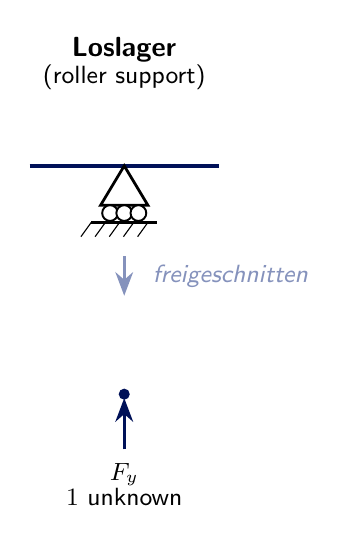
\begin{tikzpicture}
\node[align=center] at (0,1.3) {\textbf{Loslager}\\[-2pt]\small (roller support)};
\draw[line width=1.5pt, mainblue] (-1.2,0) -- (1.2,0);
\draw[line width=1pt] (0,0) -- (-0.3,-0.5) -- (0.3,-0.5) -- cycle;
\foreach \x in {-0.18,0,0.18} {\draw[fill=white, line width=0.7pt] (\x,-0.6) circle (0.1);}
\draw[line width=1pt] (-0.42,-0.72) -- (0.42,-0.72);
\foreach \x in {-0.42,-0.24,...,0.42} {\draw[line width=0.4pt] (\x,-0.72) -- (\x-0.13,-0.9);}
\divider
\fill[mainblue] (0,-2.9) circle (2pt);
\draw[force] (0,-3.6) -- (0,-2.95);
\node[below] at (0,-3.65) {\small $F_y$};
\node at (0,-4.2) {\small $1$ unknown};
\end{tikzpicture}

% ================= PANEL 2: Festlager =================
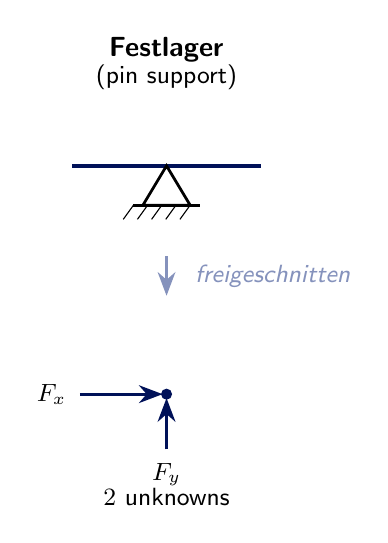
\begin{tikzpicture}
\node[align=center] at (0,1.3) {\textbf{Festlager}\\[-2pt]\small (pin support)};
\draw[line width=1.5pt, mainblue] (-1.2,0) -- (1.2,0);
\draw[line width=1pt] (0,0) -- (-0.3,-0.5) -- (0.3,-0.5) -- cycle;
\draw[line width=1pt] (-0.42,-0.5) -- (0.42,-0.5);
\foreach \x in {-0.42,-0.24,...,0.42} {\draw[line width=0.4pt] (\x,-0.5) -- (\x-0.13,-0.68);}
\divider
\fill[mainblue] (0,-2.9) circle (2pt);
\draw[force] (0,-3.6) -- (0,-2.95);
\node[below] at (0,-3.65) {\small $F_y$};
\draw[force] (-1.1,-2.9) -- (-0.05,-2.9);
\node[left] at (-1.15,-2.9) {\small $F_x$};
\node at (0,-4.2) {\small $2$ unknowns};
\end{tikzpicture}

% ================= PANEL 3: feste Einspannung =================
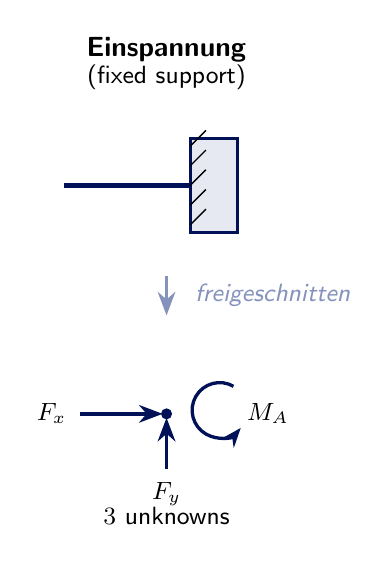
\begin{tikzpicture}
\node[align=center] at (-0.3,1.55) {\textbf{Einspannung}\\[-2pt]\small (fixed support)};
\draw[line width=1.5pt, mainblue] (-1.6,0) -- (0,0);
\fill[lightaccent, draw=mainblue, line width=1pt] (0,0.6) rectangle (0.6,-0.6);
\foreach \y in {-0.5,-0.25,...,0.5} {\draw[line width=0.5pt] (0,\y) -- (0.2,\y+0.2);}
\draw[accent, -{Stealth[length=3mm]}, line width=1pt] (-0.3,-1.15) -- (-0.3,-1.65);
\node[accent] at (1.05,-1.4) {\small \emph{freigeschnitten}};
\fill[mainblue] (-0.3,-2.9) circle (2pt);
\draw[force] (-0.3,-3.6) -- (-0.3,-2.95);
\node[below] at (-0.3,-3.65) {\small $F_y$};
\draw[force] (-1.4,-2.9) -- (-0.35,-2.9);
\node[left] at (-1.45,-2.9) {\small $F_x$};
\draw[moment, -{Stealth[length=2.5mm]}] (0.55,-2.55) arc (60:320:0.35);
\node[right] at (0.6,-2.9) {\small $M_A$};
\node at (-0.3,-4.2) {\small $3$ unknowns};
\end{tikzpicture}

% ================= PANEL 4: Fuehrung, horizontal sliding (Fy + M) =================
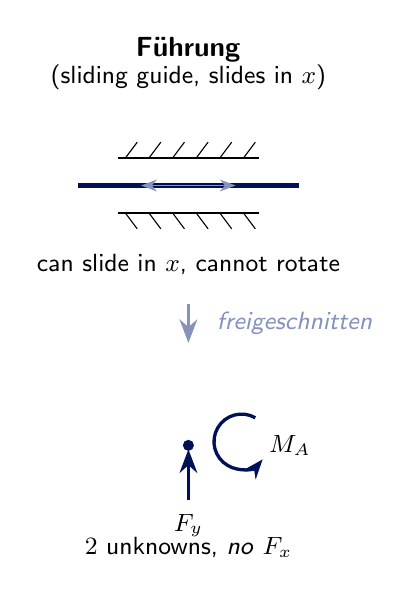
\begin{tikzpicture}
\node[align=center] at (0,1.55) {\textbf{F\"uhrung}\\[-2pt]\small (sliding guide, slides in $x$)};
\draw[line width=1.5pt, mainblue] (-1.4,0) -- (1.4,0);
\draw[line width=1pt] (-0.9,0.35) -- (0.9,0.35);
\draw[line width=1pt] (-0.9,-0.35) -- (0.9,-0.35);
\foreach \x in {-0.8,-0.5,...,0.8} {\draw[line width=0.4pt] (\x,0.35) -- (\x+0.15,0.55);}
\foreach \x in {-0.8,-0.5,...,0.8} {\draw[line width=0.4pt] (\x,-0.35) -- (\x+0.15,-0.55);}
\draw[dim, {Stealth[length=2mm]}-{Stealth[length=2mm]}] (-0.6,0) -- (0.6,0);
\node[align=center] at (0,-1.0) {\small can slide in $x$, cannot rotate};
\draw[accent, -{Stealth[length=3mm]}, line width=1pt] (0,-1.5) -- (0,-2.0);
\node[accent] at (1.35,-1.75) {\small \emph{freigeschnitten}};
\fill[mainblue] (0,-3.3) circle (2pt);
\draw[force] (0,-4.0) -- (0,-3.35);
\node[below] at (0,-4.05) {\small $F_y$};
\draw[moment, -{Stealth[length=2.5mm]}] (0.85,-2.95) arc (60:320:0.35);
\node[right] at (0.9,-3.3) {\small $M_A$};
\node at (0,-4.6) {\small $2$ unknowns, \emph{no} $F_x$};
\end{tikzpicture}

% ================= PANEL 5: Fuehrung, vertical sliding (Fx + M) =================
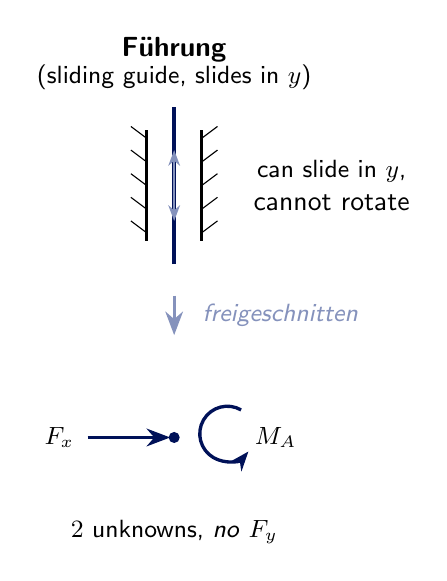
\begin{tikzpicture}
\node[align=center] at (0,1.55) {\textbf{F\"uhrung}\\[-2pt]\small (sliding guide, slides in $y$)};
\draw[line width=1.5pt, mainblue] (0,-1.0) -- (0,1.0);
\draw[line width=1pt] (0.35,-0.7) -- (0.35,0.7);
\draw[line width=1pt] (-0.35,-0.7) -- (-0.35,0.7);
\foreach \y in {-0.6,-0.3,...,0.6} {\draw[line width=0.4pt] (0.35,\y) -- (0.55,\y+0.15);}
\foreach \y in {-0.6,-0.3,...,0.6} {\draw[line width=0.4pt] (-0.35,\y) -- (-0.55,\y+0.15);}
\draw[dim, {Stealth[length=2mm]}-{Stealth[length=2mm]}] (0,-0.45) -- (0,0.45);
\node[align=center] at (2.0,0) {\small can slide in $y$,\\ cannot rotate};
\draw[accent, -{Stealth[length=3mm]}, line width=1pt] (0,-1.4) -- (0,-1.9);
\node[accent] at (1.35,-1.65) {\small \emph{freigeschnitten}};
\fill[mainblue] (0,-3.2) circle (2pt);
\draw[force] (-1.1,-3.2) -- (-0.05,-3.2);
\node[left] at (-1.15,-3.2) {\small $F_x$};
\draw[moment, -{Stealth[length=2.5mm]}] (0.85,-2.85) arc (60:320:0.35);
\node[right] at (0.9,-3.2) {\small $M_A$};
\node at (0,-4.4) {\small $2$ unknowns, \emph{no} $F_y$};
\end{tikzpicture}

% ================= PANEL 6: Pendelstuetze at an angle =================
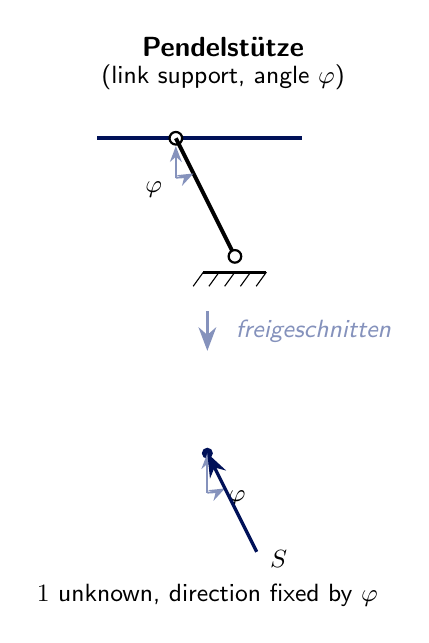
\begin{tikzpicture}
\node[align=center] at (0.6,2.15) {\textbf{Pendelst\"utze}\\[-2pt]\small (link support, angle $\varphi$)};
\draw[line width=1.5pt, mainblue] (-1.0,1.2) -- (1.6,1.2);
\draw[fill=white, line width=0.8pt] (0,1.2) circle (0.08);
\draw[line width=1.4pt] (0,1.2) -- (0.75,-0.3);
\draw[fill=white, line width=0.8pt] (0.75,-0.3) circle (0.08);
\draw[line width=1pt] (0.35,-0.5) -- (1.15,-0.5);
\foreach \x in {0.35,0.55,...,1.15} {\draw[line width=0.4pt] (\x,-0.5) -- (\x-0.13,-0.68);}
\draw[dim] (0,0.7) -- (0,1.1);
\draw[dim] (0,0.7) arc (270:296.6:0.5);
\node[left] at (-0.05,0.55) {\small $\varphi$};
\draw[accent, -{Stealth[length=3mm]}, line width=1pt] (0.4,-1.0) -- (0.4,-1.5);
\node[accent] at (1.75,-1.25) {\small \emph{freigeschnitten}};
\fill[mainblue] (0.4,-2.8) circle (2pt);
\draw[dim] (0.4,-3.3) -- (0.4,-2.8);
\draw[dim] (0.4,-3.3) arc (270:296.6:0.5);
\node[below right] at (0.55,-3.15) {\small $\varphi$};
\draw[force] ($(0.4,-2.8)+(-63.4:1.4)$) -- (0.4,-2.8);
\node[right] at ($(0.4,-2.8)+(-63.4:1.5)$) {\small $S$};
\node at (0.4,-4.6) {\small $1$ unknown, direction fixed by $\varphi$};
\end{tikzpicture}

\end{document}
